% OUTLINE
% 1. Purpose of the chapter
% 2. Overview of the socket wrapper library
% 3. Plus one service
% 3.1 Server Description
% 3.2 Client Description
% 3.3 Running client and server
% 4. Survey Service
% 4.1 Support functions
% 4.2 Server description
% 4.3 Client description
% 4.4 Running client and server
% 5 Enhanced server
% 5.1 SocketAddress
% 5.2 iostream interface
% 5.3 Server description
% 5.4 Client description
% 5.5 Administrative client description
% 5.6 Running server and the clients
	
\chapter{Socket Programming in C++}
\label{chap:cpp}

\vspace{-0.3in}
\textbf{(contributed by David B.\ Sturgill)}

\vspace{-0.2in}
{\Large {\bf David B. Sturgill}}
\vspace{0.3in}

This book is for people who want to understand sockets.  It's for
people who want to know not only how to get a couple of programs to
communicate over a network but also how and why the sockets API works
like it does.  Or course, lots of developers use sockets all the time
without really understanding these details.  It's common to use
sockets via a library that offers a simplified interface to socket
creation, name resolution and message transmission.  This is
particularly common in object-oriented languages like C++ and Java,
where it's easy to wrap socket functionality in a collection of
related classes.

The PracticalSocket library was developed to help expose students to
the basics of socket programming without requiring a complete
understanding of some of the material covered elsewhere in this book.
This library is typical of object-oriented wrappers around socket
functionality; it tries to offer a simple interface to the most
commonly used functionality.  The PracticalSocket library provides
portability between Windows and Unix platforms, and it can serve an
instructional purpose since its source code is readily available.

A reader who is more comfortable in C or who prefers to start by
understanding what's going on underneath should save this chapter for
last.  It can serve as a summary and application of many of the
concepts introduced earlier.  For a reader who is an experienced C++
programmer or who prefers to learn about sockets more selectively,
this chapter can be read earlier and can serve as an overview of
concepts covered in much more detail in earlier chapters.  The
examples presented here include many pointers to appropriate sections
earlier in the text, so this chapter can serve as an entry point for
many other sections of the book.

In this chapter, we introduce the PracticalSocket library and
demonstrate its use in a simple application.  Through a series of more
sophisticated applications, we expose additional features of the
library and demonstrate how PracticalSockets or a similar library
might be used in practice.  Both the PracticalSocket library and the
example programs used in this chapter to demonstrate it are available
from the website for this text.

\section{PracticalSocket Library Overview}

\noindent
Figure~\ref{fig:Inheritance} illustrates the classes in
PracticalSockets and their inheritance relationships.  All the classes
ending in ``Socket'' serve as wrappers around TCP or UDP sockets and
provide a simple interface for creating a socket and using it for
communication.  The \type{SocketException} class provides support for
error handling, and \type{SocketAddress} serves as a wrapper around an
address and port number.

\begin{figure}[htbp]
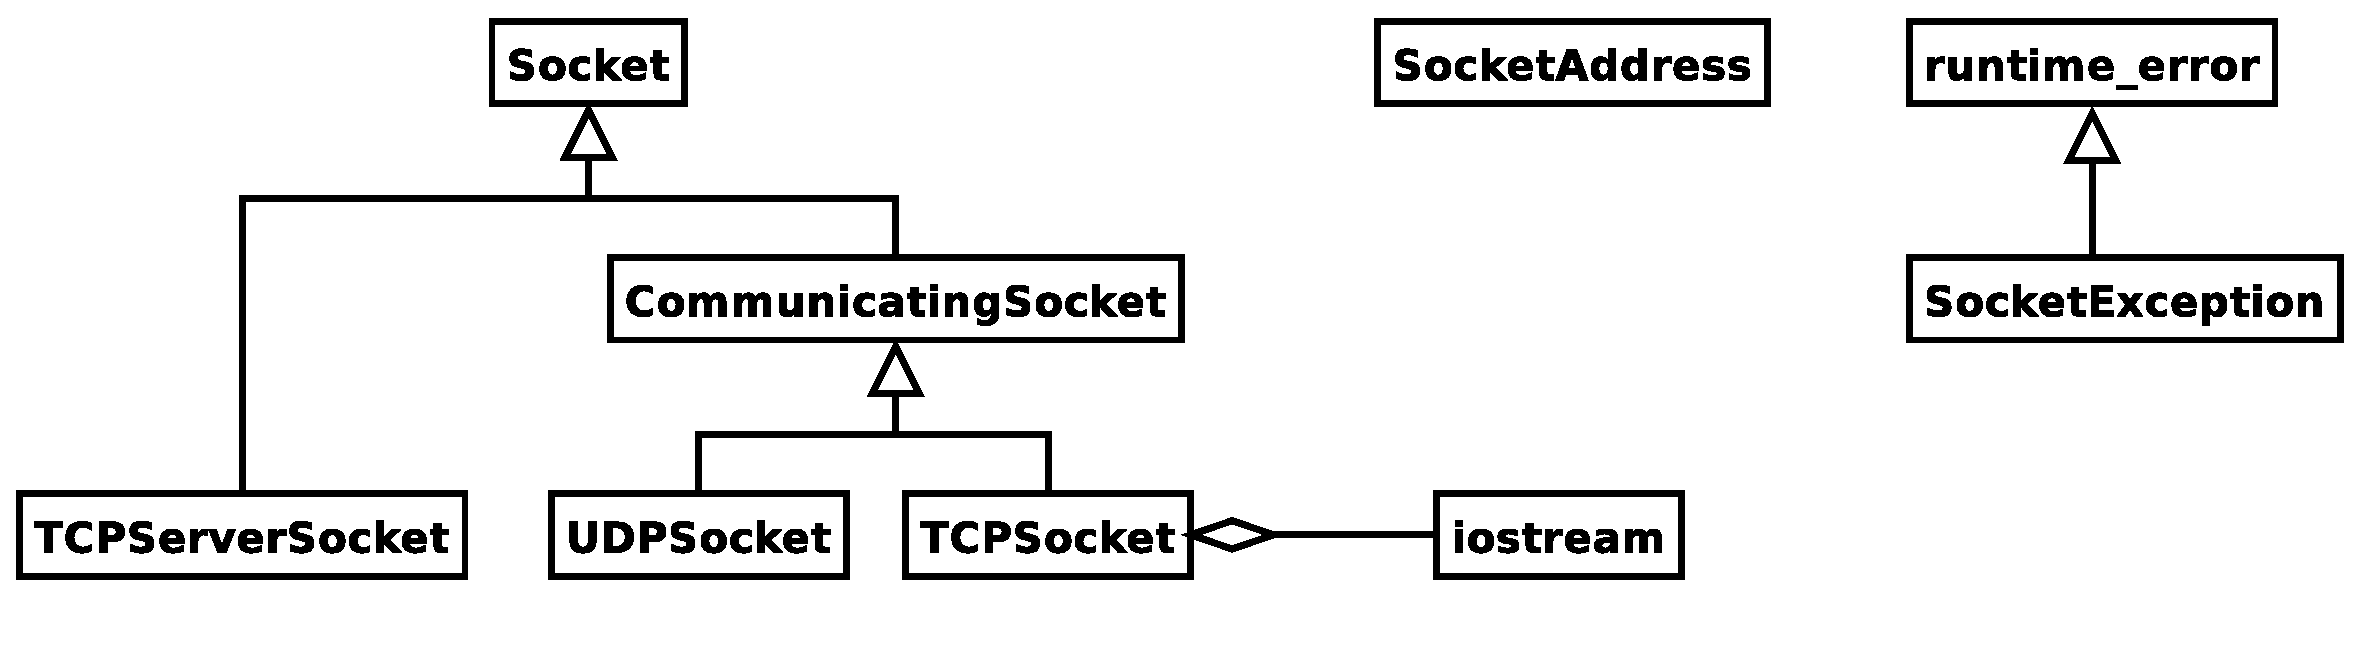
\includegraphics[width=5.5in]{figures/Inheritance.eps}
\caption{\label{fig:Inheritance}PracticalSockets Class Diagram}
\end{figure}

We can get started using this library without understanding everything
about its classes and methods all at once.  We'll start by covering
just enough to write a simple application.  From there, we can
introduce new features gradually.

The \type{TCPSocket} class is the basic mechanism for communication
over TCP.  It is implemented as wrapper around a TCP socket and serves
as an endpoint in a bidirectional communication channel.  If two
applications want to communicate, they can each obtain an instance of
\type{TCPSocket}.  Once these two sockets are connected, sequences of
bytes sent from one can be received at the other.

Functionality for \type{TCPSocket} is distributed across the class
itself and its two base classes, \type{CommunicatingSocket} and
\type{Socket}.  The \type{Socket} class is at the top of the
inheritance hierarchy, and contains only functionality common to all
socket wrappers.  Among other things, it has the job of keeping up
with the underlying socket descriptor, and it automatically closes its
descriptor when it is destroyed.

The \type{CommunicatingSocket} class is an abstraction for a socket
that, once connected, can exchange data with a peer socket.  It
provides \fcnref{send()} and \fcnref{recv()} methods that are wrappers
around the \fcnrefsys{send()} and \fcnrefsys{recv()} calls for the
underlying socket descriptor.  A successful call to the
\fcnref{send()} method of a \type{CommunicatingSocket} will send the
first \param{bufferLen} bytes pointed to by \param{buffer} to the peer
\type{CommunicatingSocket}.  A call to the \fcnref{recv()} method of a
\type{CommunicatingSocket} will attempt to read up to
\param{bufferLen} bytes of data from the peer and store the result in
the memory pointed to by \param{buffer}.  The \fcnref{recv()} method
will block until data is available on the socket, and it will return
the number of bytes received on the socket and written into \param{buffer}.
After a socket is closed, \fcnref{recv()} will return zero to indicate
that no more data can be received.

\begin{inlinefcn}
\type{void} \type{CommunicatingSocket}::\fcnref{send}(\type{const void *}\param{buffer},
\type{int} \param{bufferLen}) throw(\type{SocketException});\\
\type{int} \type{CommunicatingSocket}::\fcnref{recv}(\type{void *}\param{buffer}, \type{int}
\param{bufferLen}) throw(\type{SocketException});\\
\type{int} \type{CommunicatingSocket}::\fcnref{recvFully}(\type{void *}\param{buffer}, \type{int}
\param{bufferLen}) throw(\type{SocketException});
\end{inlinefcn}

The stream of bytes transmitted between sockets may be fragmented into
packets and reconstituted by buffering on its way from the sender to
the receiver.  \callout{A group of bytes sent in a single call to
\fcnref{send()} may not all be received in a single, corresponding
call to \fcnref{recv()}}.  The \fcnref{recvFully()} method is intended
to help with this.  It works just like \fcnref{recv()}, except that it
blocks until either exactly \param{bufferLen} bytes are received or
the socket is closed.  The return value from \fcnref{recvFully()}
reports the number of bytes received.  Ordinarily, this will be the
same as \param{bufferLen}.  However, if the socket is closed before
all the requested bytes are transmitted, a value less than
\param{bufferLen} may be returned.

The PracticalSocket library uses C++ exceptions to report when
something goes wrong.  This is evident in the prototypes above.  An
instance of \type{SocketException} is thrown whenever an error occurs
in the library.  This exception object inherits from
\typesys{runtime\_error}, so it can be caught as an instance of
\type{SocketException} by error handling code specific to the
communications portion of an application.  A \type{SocketException}
may be caught as a more general exception type by more general
error-handling code.  The \fcnrefsys{what()} method of a
\type{SocketException} returns a string with a short description of
the particular error that occurred.

The way to obtain an instance of \type{TCPSocket} depends on the role
of the application.  To establish a pair of connected \type{TCPSocket}
peers, one application must function as a server and the other as a
client.  The server listens for new connections by creating an
instance of \type{TCPServerSocket}.  The other creates a
\type{TCPSocket} directly.  The \type{TCPServerSocket} class is
derived from \type{Socket}, but not \type{CommunicatingSocket}.  It is
used to establish new TCP socket connections with client applications,
but isn't, itself, used to send and receive bytes.  The server must
construct a \type{TCPServerSocket} with an application-defined port
number.  Afterward, a call to \fcnref{accept()} will block until a
client application attempts to connect by creating a \type{TCPSocket}
with the same port number.  When this happens, \fcnref{accept()}
will return a pointer to a new instance of \type{TCPSocket} that is
connected to the \type{TCPSocket} peer on the client.

\begin{inlinefcn}
\fcnref{TCPServerSocket}(\type{unsigned short}localPort) 
      throw(\type{SocketException});\\
\type{TCPSocket *}\type{TCPServerSocket}::\fcnref{accept}() 
throw(\type{SocketException});
\end{inlinefcn}

The client application creates its end of the socket connection by
simply constructing an instance of \type{TCPSocket} and providing the
name or address of the server's host and the same port number.  Once a
pair of connected \type{TCPSocket} objects have been created, client
and server can communicate using the \fcnref{send()} and
\fcnref{recv()} methods until one of the endpoints closes its
connection via the destructor or the \fcnref{close()} method.

\begin{inlinefcn}
\fcnref{TCPSocket}(\type{const char *}\param{foreignAddress},
\type{in\_port\_t} \param{foreignPort})
throw(\param{SocketException});\\
\type{void} \type{Socket}::\fcnref{close}();
\end{inlinefcn}

\section{Plus One Service}

The few classes and methods introduced so far are enough to let us
implement a simple client and server similar to the ones in previous
chapters.  Here, accessing sockets through the PracticalSocket
classes yields somewhat shorter source code that hides many of the
details of the underlying API.  The ``plus one'' service is a
client-server application that performs the increment operation.  The client
sends an unsigned integer to the server and the server sends back a
value that's one greater.

\subsection{Plus One Server}

\file{PlusOneServer.c} is the server portion of the application.  It
accepts client connections, reads a 32-bit unsigned integer from each
client, increments it and then sends it back.

\jcode{PlusOneServer.cpp}{practical/PlusOneServer.cpp}{1}{1}

\begin{topcode}


\tlcitems{Application setup}{1--6}

Access to the sockets API is hidden behind the PracticalSocket
classes.  The application only needs to include the header for the
library and any calls we use directly.


\tlcitems{Error handling}{8, 25--27}

Error handling is via exceptions.  If an error occurs, it is caught at
the end of the main function, and the program prints an error message
before terminating.

\tlcitem{Create a server socket}{9}

The server creates a \type{TCPServerSocket} that listens for
connections on port 9431.  When constructed like this, the
\type{TCPServerSocket} automatically makes the calls to
\fcnref{socket()}, \fcnref{bind()} and \fcnref{listen()} described in
Sections~\ref{sect:connectingASocket}, \ref{sect:bindingToAnAddress}
and \ref{sect:handlingIncomingConnections}.  If anything goes wrong in
one of these steps, an exception is thrown.

To keep the example simple, the server's port number is hard-coded in
the constructor call.  Of course, it would be more maintainable to use
a named constant in a header file as the port number.

\tlcitems{Repeatedly accept client connections}{12--13}

The server repeatedly calls the \fcnref{accept()} method to wait for a
new client connection.  When a client connects, this method returns a
pointer to a new \type{TCPSocket} for communicating with the client.
This method is a wrapper around the \fcnref{accept()} call described
in Section~\ref{sect:handlingIncomingConnections}.  If something goes
wrong in \fcnref{accept()}, the catch block reports the error and the
program terminates.

\tlcitems{Read an integer from the client and convert byte order}{15--17}

Client and server have been written to exchange fixed-sized messages
in the form of unsigned 32-bit integers.  The server uses a
stack-allocated integer, \var{val}, to hold the received message.
Since the server is expecting a four-byte message, it uses the
\fcnref{recvFully()} method of \type{TCPSocket} to read the message
directly into the storage for \var{val}.  If the client connection is
closed before the entire message arrives, \fcnref{recvFully()} returns
fewer than the expected number of bytes and the server ignores the
message.

Although client and server agree on the size of a message, if they are
running on different hosts, they may represent integers using
different byte orders.  To take care of this possibility, we agree to
only transmit values that are in big-endian byte order.  The server
uses \fcnref{ntohl()} to convert the received integer to local byte
order if necessary.  

Concerns over reading entire messages and adjusting byte order are
really just the issues of framing and encoding.
Chapter~\ref{chap:encoding} focuses specifically on these topics and
offers a variety of techniques for handling framing and encoding.

\tlcitems{Increment the client integer and send it back}{18--20}

The server adds one to the client-provided value and then converts it
back to network byte order.  The server sends the value back to
the client by sending a copy of the four bytes of memory used to
represent \var{val}.

\tlcitem{Close client connection}{22}

When the server destroys its instance of \type{TCPSocket}, the
socket connection is closed.  If the server had neglected
to destroy this object, it would have not only leaked memory but also
leaked an underlying socket descriptor with each client connection.  A
server with this type of bug could very quickly reach an
operating-system-enforced limit on per-process resources.

\end{topcode}

\subsection{Plus One Client}

\file{PlusOneClient.c} is the client counterpart of the plus one
server.  It connects to the server, sends it a copy of an integer
value given on the command line, and prints out the value the server
sends back.

\jcode{PlusOneClient.cpp}{practical/PlusOneClient.cpp}{1}{1}

\begin{topcode}

\tlcitems{Application setup and parameter checking}{1--12}

The client uses the PracticalSocket classes along with support from a
few other header files.  On the command line, the client expects an
address or hostname for the server and an integer value to send to the
server.  A usage message is printed if the wrong number of arguments is given.

\tlcitems{Error handling}{14, 27--29}

As in the server, a socket-related exception is caught by code at the
end of the program, and an error message is printed.

\tlcitem{Connect to the server}{14}

The client creates an instance of \type{TCPSocket}, passing in the
user-supplied hostname and the hard-coded port number for the server.
This constructor hides a lot of detail in the underlying sockets API.
First, the given hostname is resolved to one or more addresses.  As
<<<<<<< cpp.tex
described in Chapter~\ref{sect:address-independence}, the
=======
described in Chapter~\ref{chap:addrindep}, 
>>>>>>> 1.6
\fcnref{getaddrinfo()} returns all matching addresses for a given host
and port.  Some may be IPv4 addresses, and some may be IPv6.  The
\type{TCPSocket} constructor creates a socket for the first address and
attempts to connect to it.  If this fails, each successive address is
tried until a connection can be established.  If no addresses will
connect, an exception is thrown.

\tlcitems{Parse, convert and send value to server}{17--19}

The client parses the user-provided value from the command line,
converts it to network byte order and sends it to the server by
sending the four bytes starting at the value's starting address.


\tlcitems{Receive incremented value, convert and print}{22--25}

Using \fcnref{recvFully()}, the client blocks until it either receives a
four-byte integer from the server or the socket connection is closed.
If all four bytes arrive, the received value is converted to
host byte order and printed.

\tlcitem{Close the socket}{25}

Since the client's \type{TCPSocket} is allocated on the stack, it is
automatically closed and destroyed when the socket goes out of scope.

\end{topcode}

\subsection{Running Server and Client}

The executable \exec{PlusOneServer} requires no command-line
arguments.  Once compiled, it should be started from the command
prompt and permitted to run for as long as you want to try it out.
While the server is running, you should run a copy of
\exec{PlusOneClient} from a different command prompt, possibly on a
different host.  Supply the name of the server's host and an integer
value on the command line and it should, with a little help from the
server, produce a value one larger than the command-line argument.
For example, if the server is running on a host named ``venus,'' you
should be able to run the client as follows:

\noindent \textbf{PlusOneClient connecting to a server on host, venus}
\begin{shell}
\prompt \typed{PlusOneClient venus 345318} \\
\response{Server Response: 345319}
\end{shell}

\begin{exercises}

\item Instead of simply incrementing the value from a single client,
  modify the server so it will send back the sum of two values
  supplied by different clients.  After a first client connects, the
  server will wait for a second client.  The server will read integer
  values from both clients and send back the sum of these two values
  to both.

\item The client and server communicate using binary-encoded,
  fixed-sized messages.  Modify these programs so that they use
  variable-length, text-encoded messages as described in
  Section~\ref{sect:textEncoding}.  The sender will write its integer
  value to character array as a sequence of ascii-encoded digits.  The
  receiver will read a copy of this array and parse out the integer.

\end{exercises}

\section{Survey Service}

Building on the concepts demonstrated in the plus one service and
using techniques presented in Chapters~\ref{chap:encoding} and
\ref{chap:advanced}, we can create a distributed application that does
something a little more useful.  The survey client and server
implement a simple, distributed survey application.  At startup, the
server reads a list of survey questions and responses from a text
file.  When a client connects, the server sends it copies of the
questions and response options.  The client prints each question and
sends the user's response back to the server, where it is recorded.

The file, \file{survey1.txt}, is an example survey file the server
might use.  The first line gives the number of questions.  This is
followed by a description for each question.  A question is described
by a one-line prompt, followed by a line giving the number of
responses and a line of text for each response.  For example, the
first question on the survey below is ``What is your favorite flavor
of ice cream?''  The three possible responses are ``Vanilla,''
``Chocolate'' or ``Strawberry.''  As users take the survey, the server
will keep up with how many selected each of these responses.

\jcode{survey1.txt}{practical/survey1.txt}{1}{1}

\subsection{Survey Support Functions}

The client and server depend on common functionality implemented in
\file{SurveyCommon.h} and \file{SurveyCommon.cpp}.  The header file
provides a named constant for the server's port number, a
\type{Question} type for representing survey questions and prototypes
for provided functions.

\jcode{SurveyCommon.h}{practical/SurveyCommon.h}{1}{1}

\jcode{SurveyCommon.cpp}{practical/SurveyCommon.cpp}{1}{1}

\begin{topcode}

\tlcitems{Integer encode and decode}{5--8, 16-22}

In this application, client and server communicate by exchanging
values of type integer and string.  Integers are handled much like
they are in the plus one service.  To encode a 32-bit integer, it is
first converted to network byte order and then sent out over a socket.
To receive an integer, we attempt to read four bytes from the socket
and, if successful, convert them to host byte order and return the
result.  If four bytes can't be read, an exception is thrown.  Since
this type of error is not produced in the PracticalSocket library
itself, the exception is reported as a \type{runtime\_error} rather
than a \type{SocketException}.

\tlcitems{String encode and decode}{10--14, 24--37}

Encoding and decoding of strings is more complicated because they can
be of arbitrary length.  Strings are encoded by first sending the
string length and following this by the content of the string.  The
decoder tries to read both of these values and, if successful,
converts the received string contents to a \type{string} object and
returns it.

\tlcitems{Parse survey}{38-59}

The survey is stored in a text file.  The \fcnref{readSurvey()} function
reads the survey from the given input stream and fills in the given
\var{qList} parameter with the sequence of questions.

\end{topcode}

\subsection{Survey Server}

The survey server is responsible for maintaining the list of survey
questions, keeping up with user response totals and interacting with
the client.

The plus one server was able to handle only one client connection at a
time.  If multiple clients wanted to use the service, they would have
to take turns.  As discussed in Chapter~\ref{chap:advanced},
\Sect{sect:multiplexing}, this makes sense a simple application where
we can expect very short exchanges with each client.  However, it may not
work for the survey service.  Here, users may deliberate for
as long as they want over each question.  If two users want to take
the survey at the same time, it wouldn't be reasonable to make one
wait until the other is finished.

To interact with more than one client at the same time, the survey
server creates a separate thread to handle interaction with each
client.  As in Section~\ref{sect:perClientThread}, the new thread
manages the session with the client.  Each time the server receives a
response, it tallies it in its response count.  Mutual exclusion helps
the server to make sure two threads don't modify the response totals
at the same time.

\jcode{SurveyServer.cpp}{practical/SurveyServer.cpp}{1}{1}

\begin{topcode}

\tlcitems{Access to library functions}{1--6}

The server uses standard C++ I/O facilities and POSIX threads for
interacting with multiple concurrent clients.

\tlcitems{Survey representation}{9--11}

The survey is represented as a \type{vector} of \type{Question}
instances.  The variable, \var{rCount} keeps up with user response
counts, with each element of \var{rCount} corresponding to a survey
question.  Since each question has several possible responses, each
element of \var{rCount} is a \type{vector} of totals, one for each
response.  Each time a user selects a response, the count for that
question and response is incremented.

If multiple clients connect to the server at the same time, it's
possible that two or more of them will try to increment a counter at
the same time.  Depending on how this increment is performed by the
hardware, this could leave the count in an unknown state.  For example,
an increment performed in one thread might overwrite the result of an
increment that was just completed in another thread.  The chances of
this happening are remote, but this possibility should not be left to
chance.  The \var{lock} variable is a mutex that is used to manage
concurrent access to \var{rCount}.  Using this synchronization object,
it will be easy to make sure only one thread at a time tries to modify
\var{rCount}.

The server uses file-scoped variables to keep up with the survey and
responses.  This makes it easy to access these data structures from
any of our threads.  Using the static modifier prevents these
variables from polluting the global namespace, since they are only
visible to a single implementation file.  However, this organization
would be an impediment to code reuse if, say, we wanted to run
multiple surveys from the same application.

\tlcitems{Initialize server state}{17--31}

The server parses the survey text from a user-supplied file.  If
anything goes wrong during this process, an error message is printed
and the server exits.  After the \type{Question} list has been
successfully read, we know how many questions and responses there are,
so we initialize the parallel response count representation.  The
mutex, \var{lock}, must also be initialized before it can be used.

\tlcitems{Create server socket and repeatedly accept clients}{35--45}

The server creates a \type{TCPServerSocket} listening on an
agreed-upon port number.  It repeatedly waits for client connections,
and for each connection creates a new thread to handle interaction
with the client.  When creating the thread, the server gives a pointer
to the \fcnref{conductSurvey} function as the starting point for the new thread
and a pointer to the new \type{TCPSocket} as the thread's argument.  From this
point on, the new thread is responsible for the socket object and for
interacting with the client.  Of course, if a new thread can't be
created, the server prints an error message and cleans up by deleting
the socket immediately.

\tlcitems{Thread startup}{53--54}

The \fcnref{conductSurvey} function serves as the main function for
each new thread.  The thread will execute this function once it starts
up, and it will terminate once it returns out of the function.  The
parameter and return types of this function are determined by the
Pthreads API.  The void pointers are intended to let us pass 
pointers to any type of data we need.  Here, we know we passed in a
pointer to a \type{TCPSocket} instance, so the first thing we do is
cast it to a more specific type to make it easier to use.

Depending on the number of clients connecting, there may be several
copies of \fcnref{conductSurvey} running at the same time, each on its
own thread.  While all of these threads may be running in the same
function, each has its own local variables, and each is communicating
over the instance of \type{TCPSocket} that was provided at thread
startup.

\tlcitems{Survey client handler}{53--79}

\begin{bottomcode}

\blcitems{Send each question to client}{56--63}

The server uses functions provided by \file{SurveyCommon.cpp} to
simplify interaction with the client.  It sends the client the number
of questions in the survey and then sends each question and its
response list after the client as answered the previous question.

\blcitems{Get client response and tally it}{66--71}

The client indicates the user's chosen response by sending its index
back to the server.  Before tallying the response, the server makes
sure it's in the range of legitimate responses.  This check is very
important.  If the server incremented in \var{rCount} using an
arbitrary client-supplied index, it would be giving the client
permission to make changes at unknown memory locations.  A malicious
client could use this to try to crash the server or, worse, take
control of the server's host.  Of course, we wrote the client and the
server code.  You will see that we perform a similar check on the
client before we even send a response, so what's the point of also
performing the check on the server?  We're not concerned about the
behavior of properly-functioning clients.  We're more concerned about
what will happen if a malicious user creates a client that doesn't
behave as nicely as the one we wrote.

If a legitimate response is received, the client thread locks the
mutex to make sure no other threads are trying to modify \var{rCount}
at the same time.  It then increments the appropriate count and
unlocks the mutex right away to let other threads make changes to
\var{rCount} as needed.  This is typical of the operation of a
multi-threaded application.  In general, we want to lock out other
threads for as short a period as possible.  Consider what would happen
if threads locked the mutex once at the start of
\fcnref{conductSurvey} and then released it when they were done.  This
would eliminate the need to lock and unlock the mutex on every
response, but it would completely suppress concurrency; only one
thread at a time could interact with its client.

\blcitems{Error handling}{55,73--75}

An exception occurring in the client thread will terminate the thread,
but the server will continue to run and accept new connections.  This
makes sense as such an exception may simply result from a client
terminating unexpectedly.  If an exception is caught during client
interaction, execution falls through to the thread exit code.  Note
that the exception is caught as the more general type,
\type{runtime\_exception}, since it may be thrown either by
PracticalSockets or by our own \fcnref{recvInt()} or
\fcnref{recvString()} functions.

\blcitems{Close socket and exit}{77--78}

Since the thread in \fcnref{conductSurvey} is responsible for its
dynamically allocated \type{TCPClient} instance, it must free the
instance before it exits.  Like a C++ stream, deleting the object
automatically closes the underlying socket.

\end{bottomcode}

\end{topcode}

\subsection{Survey Client}

The survey client is not as complicated as its server.  Here, we
don't have to worry about multi-threading, concurrency or maintaining
response counts.  

\jcode{SurveyClient.cpp}{practical/SurveyClient.cpp}{1}{1}

\begin{topcode}

\tlcitems{Access to library functions}{1--4}

\tlcitems{Connect to server}{9--12}

The client expects the hostname of the server on the command line.  If
it's not given, an error message is printed and the client exits.  The
client attempts to create a \type{TCPSocket} object using the hostname
and the server's port number defined in \file{SurveyCommon.h}.  If a
connection can't be established, the exception handling code will
report an error and exit.

\tlcitems{Receive and print survey questions}{18--25}

Using functions provided by \file{SurveyCommon.cpp}, the client reads
the number of questions and then reads each question and its list of
responses.

\tlcitems{Read user responses and send them to the server}{28--35}

For each question, the user is prompted for a response.
The client checks to make sure the response is in the proper range
before sending it to the server.

\end{topcode}

\subsection{Running Server and Client}

The \exec{SurveyServer} requires one command-line argument, the name
of the file containing the survey questions.  For a survey file like
the one above, we can run the server like:

\noindent \textbf{SurveyServer offering questions from \texttt{survey1.txt}}
\begin{shell}
\prompt \typed{SurveyServer survey1.txt} \\
\end{shell}

\noindent
The \exec{SurveyClient} requires one command-line argument, the
server's hostname or address.  If the server is running on a system
named ``earth,'' we could run the client as:

\noindent \textbf{SurveyClient connecting to a server on host, earth}
\begin{shell}
\prompt \typed{SurveyClient earth} \\
\response{Q0:  What is your favorite flavor of ice cream?}\\
\response{ 0 Vanilla}\\
\response{ 1 Chocolate}\\
\response{ 2 Strawberry}\\
\response{> }\\
\end{shell}

\noindent
From this point, the user can respond to questions by entering the
index of the desired response.  The client terminates once all
questions have been answered.

\section{Survey Service, Mark 2}

Although it performs a modestly useful function as it is, the survey
service is ripe for enhancement.  In this section, we add an
administrative interface to report on response counts, we have the
server keep a list of IP addresses of clients completing the survey,
and we explore an alternative technique for encoding and decoding
messages between client and server.  A few additional features of the
PracticalSocket library are needed to make these enhancements to the
survey service.

\subsection{Socket Address Support}

The PracticalSocket library provides a \type{SocketAddress} class that
encapsulates an IP address and a port number.  It's actually just a
wrapper around the \type{sockaddr\_storage} structure introduced in
Section~\ref{sect:specifyingAddresses}.  Objects of this type are
handy for keeping up with the endpoints of a socket connection and the
library uses them in many different places.

Through its constructors and static \fcnref{lookupAddresses()} methods,
\type{SocketAddress} provides a simple interface to name resolution.
An instance of SocketAddress can be constructed with either an address
or a hostname and a port number.  Alternatively, the port can be
described using a service name instead of a number.  Both of these
constructors are wrappers around the \fcnrefsys{getaddrinfo()} function
described in Chapter~\ref{chap:addrindep}.  The underlying
\fcnrefsys{getaddrinfo()} actually returns a list of matching
addresses, and these constructors simply use the first address that's
returned.  The static \fcnref{lookupAddresses()} methods take the same
parameters as these constructors and return a list of all matching
addresses in an STL \type{vector}.  This could be useful for an
application that needs to choose between IPv4 or IPv6 or when multiple
network interfaces are available on a single host.

\begin{inlinefcn}
\fcnref{SocketAddress}(\type{const char *}\param{host},
\type{in\_port\_t} \param{port})
throw(\type{SocketException});\\ 
\fcnref{SocketAddress}(\type{const char
  *}\param{host}, \type{const char *}\param{service})
throw(\type{SocketException});\\ 
static \type{std::vector$\langle$SocketAddress$\rangle$}
\type{SocketAddress}::\fcnref{lookupAddresses}(\type{const char
  *}\param{host},\\
\hspace*{2in}\type{in\_port\_t} \param{port}) throw(\type{SocketException});\\
static \type{std::vector$\langle$SocketAddress$\rangle$}
\fcnref{lookupAddresses}(\type{const char *}\param{host},\\
\hspace*{2in} \type{const char *}\param{service})
 throw(\type{SocketException});\\
\end{inlinefcn}

Instances of \type{SocketAddress} can also be obtained by querying the
addresses at the ends of a socket connection.  The base class,
\type{Socket}, provides a \fcnref{getLocalAddress()} method that
returns a \type{SocketAddress} for the local address to which a socket
is bound.  In the case of a \type{TCPServerSocket}, this will give the
address on which the server is listening, and, in the case of a
\type{TCPSocket} this will give the address at the local end of the
connection.  The \type{CommunicatingSocket} class provides a
\fcnref{getForeignAddress()} method that returns a
\type{SocketAddress} for the remote end of a connection.  Once
obtained, the host address and port number of a SocketAddress can be
examined via the \fcnref{getAddress()} and \fcnref{getPort()} methods.

\begin{inlinefcn}
\type{SocketAddress} \type{Socket}::\fcnref{getLocalAddress}()\\
\hspace*{2in} throw(\type{SocketException});\\
\type{SocketAddress}
\type{CommunicatingSocket}::\fcnref{getForeignAddress}()\\
\hspace*{2in}throw(\type{SocketException});\\
\type{std::string} \type{SocketAddress}::\fcnref{getAddress}()\\
\hspace*{2in} const throw(\type{SocketException});\\
\type{in\_port\_t} \type{SocketAddress}::\fcnref{getPort}()\\
\hspace*{2in} const throw(\type{SocketException});\\ 
\end{inlinefcn}

For the user who wants to take more control over how a socket is set
up, \fcnref{bind()} and \fcnref{connect()} methods are provided that
take an instance of \type{SocketAddress} as a parameter.  An
application can create a \type{TCPSocket} or a \type{TCPServerSocket}
using the default constructor.  The socket can then be bound to a
local address with the \fcnref{bind()} method and, in the case of
\type{TCPSocket}, connected to a remote server with the
\fcnref{connect()} method.  This lets the programmer manage socket
creation with a level of control more similar to what's described in
Chapter~\ref{chap:tcp}.

\begin{inlinefcn}
\type{void} \type{TCPSocket}::\fcnref{bind}(\type{const SocketAddress
  \&}\param{localAddress})\\
\hspace*{2in} throw(\type{SocketException});\\
\type{void} \type{TCPSocket}::\fcnref{connect}(\type{const
  SocketAddress \&}\param{foreignAddress})\\
\hspace*{2in} throw(\type{SocketException});\\
\type{void} \type{TCPServerSocket}::\fcnref{bind}(\type{const
  SocketAddress \&}\param{localAddress})\\
\hspace*{2in} throw(\type{SocketException});\\
\end{inlinefcn}

\subsection{Socket iostream Interface}

The \fcnref{send()} and \fcnref{recv()} methods provided by
\type{CommunicatingSocket} serve as a very thin veneer over the
\fcnref{send()} and \fcnref{recv()} functions for the underlying
socket.  This kind of interface is natural for some types of messages,
but it isn't the most familiar for handling text-encoded messages
as described in Section~\ref{sect:textEncoding}.  

The \fcnref{getStream()} method of \type{CommunicatingSocket} returns
a reference to an \type{iostream} that's backed by the socket.  For a
C++ programmer, this can serve as a very convenient interface for
reading and writing text-encoded information.  It's a C++ analog to
the \fcnsys{fdopen()} mechanism described in
Section~\ref{sect:streams}.  Character sequences written to the
\type{iostream} will be sent over the socket, and the sequence of
characters received from the network can be read from the
\type{iostream}.  With this interface, the programmer can use the
familiar techniques for working with \type{istream} and \type{ostream}
to encode and decode messages.

\begin{inlinefcn}
\type{std::iostream
  \&}\type{CommunicatingSocket}::\fcnref{getStream}()
throw(\type{SocketException});
\end{inlinefcn}

The \type{iostream} interface to a \type{CommunicatingSocket} provides
fixed-sized buffers for storing part of the character sequence being
sent and received.  Text written to the \type{iostream} will be held
in memory until the buffer is full or until it is flushed.  This can
offer some performance advantages since a message can be written to
the \type{iostream} one field at a time and then pushed out to the
network after it's complete.  However, this level of buffering makes
it problematic to mix I/O operations via the \type{iostream} with
direct calls to the \fcnref{send()} and \fcnref{recv()} methods.
Consider, for example, some message $A$ written to the socket via
its \type{iostream}.  If the stream isn't subsequently flushed, part
of message $A$ may remain buffered in the \type{iostream}.  If message
$B$ is then sent directly via the socket's \fcnref{send()} method, $B$
will be pushed out to the network before the buffered portions of $A$.

\subsection{Enhanced Survey Server}

The enhanced server uses \type{SocketAddress} objects to keep
up with a list of addresses for clients completing the survey.
For each client, the server records the host address by saving a
copy of the \type{SocketAddress} at the remote end of the socket.

The server also provides an administrative socket interface for
reporting the current state of the survey.  The server restricts
access to the administrative interface by only permitting connections
from clients running on the same host.  To do this, the server cannot
use the convenience constructor for \type{TCPServerSocket} used in
previous examples.  The server must create a \type{TCPServerSocket} in
the unbound state and then explicitly bind it to a
\type{SocketAddress} for the loopback interface.

The enhanced survey server makes extensive use of the
\type{iostream} interface of \type{CommunicatingSocket}.  This makes
the sending and receiving of messages look a lot like reading and
writing a file.  It also permits some additional code reuse between
the client and server.  Instead of using a new format to send survey
questions to the client, the server encodes them in the same format as
the survey file it reads at startup.  The client can use the same
\fcnref{readSurvey()} function provided by \file{SurveyCommon.cpp} to
read the list of survey questions all at once.

\jcode{SurveyServer2.cpp}{practical/SurveyServer2.cpp}{1}{1}

\begin{topcode}

\tlcitems{Access to library functions}{1--6}

\tlcitems{Survey representation}{9--11}

This version of the server adds a \type{vector} of
\type{SocketAddress} objects to keep up with the list of clients
completing the survey.  Since multiple client threads may attempt to
access this list at the same time, use of the list is protected
by the mutex, \var{lock}.

\tlcitems{Initialize server state}{23--37}

\tlcitems{Create a thread for the administrative interface}{43--46}

The server must accept connections over its primary
\type{TCPServerSocket} and its administrative
\type{TCPServerSocket}.  If the same thread tried to serve both of
these sockets, calling \fcnref{accept()} on one of them would leave it
blocked and unable to accept connections from the other.  To serve
both, the server creates a new thread to handle connections over its
administrative interface.  The \fcnref{adminServer()} function
implements this interface.

\tlcitems{Create server socket and handle each client with a new thread}{49--57}

\tlcitems{Survey client handler}{65--101}

\begin{bottomcode}

\blcitems{Encode survey and send to client}{69--78}

A client thread first writes a copy of the whole survey to the client,
using the same format as the original input file.  It uses
\fcnref{getStream()} to obtain a copy of the \type{iostream} for its
\type{TCPSocket} and then writes out the survey as if it were writing
to a file.  Instead of using \var{endl} to end each line, we use the
newline character.  Using \var{endl} would flush the stream after each
line.  As much as possible, we would like to buffer all or large portions of
the message and then send when the message is complete.  The server writes
the entire message and then calls the stream's \fcnref{flush()} method
to initiate sending of any buffered data.

\blcitems{Get client responses and tally them}{81--89}

The client has the entire survey, so the server only needs to read its
responses one after another.

\blcitems{Log the client}{92--94}

Once the client has completed the survey, the server records a copy of
its address.

\end{bottomcode}

\tlcitems{Administrative client handler}{103--143}

\begin{bottomcode}

\blcitems{Create administrative socket}{106--107}

The administrative interface uses a port number offset by one from the
survey port.  Since the server is intended to only accept
administrative connections from the local host, we have to go through
more explicit steps to construct the \type{TCPServerSocket} and bind
it to a local address.

\blcitems{Repeatedly accept administrative connections}{108--109}

Administrative clients are served with a single thread.  If two
administrative clients try to connect, the second will have
to wait for the first to be served.

\blcitems{Snapshot reported structures}{114--117}

Before sending a report, the server makes a copy of the client address
history and the response count lists.  This frees the server from
having to lock these structures repeatedly as it writes out the
report, but, more importantly, it provides a consistent snapshot of
the state.  The reported list of client addresses won't grow while the
server is printing it out.  If the server had simply locked the mutex
for the entire report generation instead of copying these lists, all
client threads would have been blocked while the server tried to send
the report to the administrative client.  A malicious administrative
client could fail to read from its socket and suspend the conducting
of surveys indefinitely.

\blcitems{Write administrative report}{119--132}

We make the server responsible for formatting the administrative
report.  It writes a tally for each question and response to the
socket's \type{iostream}, followed by the host addresses for every
client completing the survey.

\end{bottomcode}

\end{topcode}

\subsection{Enhanced Survey Client}

To communicate with the server using text-encoded messages, the client
requires a few changes.  First, instead of reading survey questions
individually, it obtains the socket's \type{iostream} and uses
\fcnref{readSurvey()} to read the whole survey at once.  The client
offers the survey to the user one question at a time and sends
corresponding responses by writing to the stream.

\jcode{SurveyClient2.cpp}{practical/SurveyClient2.cpp}{1}{1}

\subsection{Administrative Client}

A very simple client is sufficient to access the administrative
interface.  Since the server writes out the vote and client report in
a human-readable format, the client can just copy each byte it
receives from the server to the console.  The administrative client
first attempts to connect to a server running on the local host.
Since the client is attempting to connect using the administrative
port number, the server will automatically send it a report and then close
the socket connection.

The client creates a fixed-sized buffer and then copies one buffer
full after another to the console.  Even though the server writes to
the socket using its \type{iostream} interface, the socket simply
conveys the sequence of bytes written, and the client is free to read
the sequence using the \fcnref{recv()} method.  In this case,
\fcnref{recv()} is probably a more convenient interface than
\type{iostream} for echoing the server's output to the console.  The
client doesn't have to worry about how the server's report is
formatted, how many lines it contains or how long each line is.

The server's administrative report is just a sequence of printable
characters, with no null terminators anywhere in the report.  To print
out a buffer full of the report as if it was a string, the client must
mark the end of the buffer with a null terminator.  Since the
\fcnref{recv()} method returns the number of bytes successfully
saved in \var{buffer}, it's easy to fill in a null terminator at the
end.  Of course, the client has to be certain to leave room for this
extra character each time a buffer is read.  That's why the client's
call to \fcnref{recv()} advertises the buffer as one byte shorter than
its actual capacity.

\jcode{AdminClient2.cpp}{practical/AdminClient2.cpp}{1}{1}

\subsection{Running Server and Clients}

The enhanced survey server and its survey client are run with the same
arguments as the original.  The administrative client doesn't require
any arguments since it automatically tries to connect to an instance
of the survey server running on the local host at a known port number.

\begin{exercises}

\item In the server's code for the administrative interface, we made
  an effort to get a consistent snapshot of the response tally and the
  client address list before we started generating the report.
  However, since the server's \fcnref{conductSurvey()} function
  records client responses as soon as they are received, the
  administrative report may still include results for
  partially completed surveys.  Modify the server so that responses
  are tallied only after the client completes the survey.  In this
  way, both the response tallies and the list of client addresses will
  reflect only clients that actually completed the survey.

\item As it is written, it's possible for a client to cause a server
  crash.  If the client closes its socket connection while the server
  is sending it a message, the server will receive a \const{SIGPIPE}
  signal.  Consult Section~\ref{sect:signals} and modify the server so
  it will not terminate under these circumstances.

\item The survey server maintains an open socket and a thread on behalf
  of each client taking a survey.  If a client never completes the
  survey, the server never reclaims these resources.  Extend the
  server so that sockets are closed and client threads are permitted
  to terminate automatically five minutes after the client begins
  taking the survey.  When a client thread starts up, you will also
  start up another thread that we'll call the sleeper.  The sleeper
  will simply wait for five minutes and then check to see if the
  client thread is still running.  If it is, the sleeper will close
  the client's socket, which will unblock the server thread and give
  it a chance to exit.  Doing this the right way will require the server to
  maintain some additional per-client state and to perform
  some additional synchronization.  For example, a sleeper thread
  should not make a call to \fcnref{close()} if its client thread has
  already finished and deleted the socket.

\end{exercises}


